\documentclass[10pt, oneside]{article}   	% use "amsart" instead of "article" for AMSLaTeX format
\usepackage{geometry}                		% See geometry.pdf to learn the layout options. There are lots.
\geometry{letterpaper}                   		% ... or a4paper or a5paper or ... 
%\geometry{landscape}                		% Activate for for rotated page geometry
%\usepackage[parfill]{parskip}    		% Activate to begin paragraphs with an empty line rather than an indent
\usepackage{graphicx}
\usepackage{caption}
\usepackage{subcaption}
\usepackage{amssymb}
\usepackage{amsmath}
\usepackage{tikz}
\usetikzlibrary{shapes,arrows,calc,3d,chains,fit,decorations.markings}
\usepackage{circuitikz}



\begin{document}

\section{Geometry}

\tikzstyle{vecArrow} = [thick, decoration={markings,mark=at position
   1 with {\arrow[semithick]{open triangle 60}}},
   double distance=1.4pt, shorten >= 5.5pt,
   preaction = {decorate},
   postaction = {draw,line width=1.4pt, white,shorten >= 4.5pt}]
\tikzstyle{innerWhite} = [semithick, white,line width=1.4pt, shorten >= 4.5pt]

\newcommand\xorig{0}
\newcommand\hs{25}
\newcommand\ys{0}
\newcommand\yacc{0}
\newcommand\hacc{30}
\newcommand\yccc{-5}
\newcommand\hccc{30}
\newcommand\wacc{5}
\newcommand\wea{50}
\newcommand\ws{25}
\newcommand\wec{50}
\newcommand\wccc{5}
\newcommand\xacc{\xorig}
\newcommand\xea{\xacc+\wacc}
\newcommand\xs{\xea+\wea}
\newcommand\xec{\xs+\ws}
\newcommand\xccc{\xec+\wec}
\begin{tikzpicture}[scale=0.1]
\draw[thick] (\xea,\ys) -- (\xea,\ys+\hs) -- (\xea+\wea,\ys+\hs) -- (\xea+\wea,\ys) -- (\xea,\ys);
\draw[thick] (\xs ,\ys) -- (\xs ,\ys+\hs) -- (\xs +\ws ,\ys+\hs) -- (\xs +\ws ,\ys) -- (\xs ,\ys);
\draw[thick] (\xec,\ys) -- (\xec,\ys+\hs) -- (\xec+\wec,\ys+\hs) -- (\xec+\wec,\ys) -- (\xec,\ys);
\draw[thick] (\xacc,\yacc) -- (\xacc,\yacc+\hacc) -- (\xacc+\wacc,\yacc+\hacc) -- (\xacc+\wacc,\yacc) -- (\xacc,\yacc);
\draw[thick] (\xccc,\yccc+\hccc) -- (\xccc,\yccc) -- (\xccc+\wccc,\yccc) -- (\xccc+\wccc,\yccc+\hccc) -- (\xccc,\yccc+\hccc);
\draw node at (\xea +0.5*\wea ,\ys+0.5*\hs) {$\Omega^{electrode\ anode}$  };
\draw node at (\xs  +0.5*\ws  ,\ys+0.5*\hs) {$\Omega^{separator}$         };
\draw node at (\xec +0.5*\wec ,\ys+0.5*\hs) {$\Omega^{electrode\ cathode}$};
\draw node at (\xacc+0.5*\wacc,\ys+0.5*\hs) {$\Omega^{collector\ anode}$  };
\draw node at (\xccc+0.5*\wccc,\ys+0.5*\hs) {$\Omega^{collector\ cathode}$};

\draw node[anchor=south] at (\xacc+0.5*\wacc,\yacc+\hacc) {$\Gamma^{anode}$  }; 
\draw node[anchor=north] at (\xccc+0.5*\wccc,\yccc      ) {$\Gamma^{cathode}$};
\end{tikzpicture}

non overlapping domains
%$\Omega^{collector\ anode}$ 
%$\Omega^{electrode\ anode}$ 
%$\Omega^{separator}$  
%$\Omega^{electrode\ cathode}$
%$\Omega^{collector\ cathode}$
with common interfaces

define 
$\Gamma^{anode}$  
and
$\Gamma^{cathode}$  
as the two terminals of the device

\section{Governing equations}
%----------------------------------------------------------------------------- 
% ELECTROCHEMICAL
%----------------------------------------------------------------------------- 
\subsection{Electrochemical}

Governing equations for the electrolyte potential $\Phi_l$ and the solid phase
potential $\Phi_s$ are
\begin{align}
aC (\dot{\Phi}_l - \dot{\Phi}_s) &= \nabla \cdot (\sigma_l \nabla \Phi_l) \text{ on } \Omega^{electrode} \\
aC (\dot{\Phi}_s - \dot{\Phi}_l) &= \nabla \cdot (\sigma_s \nabla \Phi_s) \text{ on } \Omega^{electrode} \\
0 &= \nabla \cdot (\sigma_l \nabla \Phi_l) \text{ on } \Omega^{separator} \\
0 &= \nabla \cdot (\sigma_s \nabla \Phi_s) \text{ on } \Omega^{collector}
\end{align}
$aC$ is the specific capacitance. In our model, we assume it accounts for both 
double-layer capacitance and pseudocapacitance. $a$ is the interfacial area
per unit volume.

$\sigma_s$ and $\sigma_l$ are the electrolyte and solid phase electrical
conductivities. They are effective transport properties.

In our current model, we have
$\sigma_l=\sigma_{l0}\varepsilon^\beta$ and
$\sigma_s=\sigma_{s0}(1-\varepsilon)^\beta$.
$\varepsilon$ is the porous medium void volume fraction,
$\beta$ is the Bruggeman's coefficient (taken equal to $3/2$)...

[Interface conditions]
coming soon... (basically continuity of the fluxes within both phases)

[Boundary conditions]
arbitarily anode current collector ``grounded''
\begin{equation}
\Phi_s = 0 \text{\ on\ } \Gamma^{anode}
\end{equation}

choose from
\begin{enumerate}
\item Potentiostatic charge/discharge \\
$\Phi_s = U \text{\ on\ } \Gamma^{cathode}$
i.e. constant voltage charge/discharge

\item Galvanostatic charge/discharge \\
$\sigma_s \frac{\partial \Phi_s}{\partial n} = I / S^{cathode} \text{\ on\ } \Gamma^{cathode}$
i.e. constant current charge/discharge

\item Relaxation \\
nothing (is same as galvanostatic with zero current)

\item Constant power \\
$\Phi_s \sigma_s \frac{\partial \Phi_s}{\partial n} = P / S^{cathode} \text{\ on\ } \Gamma^{cathode}$
(nonlinear condition)
\end{enumerate}

here $S^{cathode}$ represents the surface area of the terminal on the cathode
current collector (over which we impose the current density flowing into the
device)
\begin{equation}
S^{cathode} = \int_{\Gamma^{cathode}} dS
\end{equation}

%----------------------------------------------------------------------------- 
% THERMAL
%----------------------------------------------------------------------------- 
\subsection{Thermal}

The temperature field $\Theta$ obeys
\begin{equation}
\rho C_p \dot{\Theta} = \nabla \cdot (\lambda \nabla \Theta) + q \text{ on } \Omega
\label{eq:heat_conduction}
\end{equation}
This is a standard heat conduction equation.
Material properties $\rho$, $C_p$ and $\lambda$ are density, heat capacity and
thermal conductivity.
$q=q^{reversible}+q^{irreversible}$ is the heat source.
\begin{itemize}
\item[$\diamond$] $q^{irr} = \sigma | \nabla \Phi |^2$: Joule heating (ohmic
losses $\propto R I^2$ when current traverse resistive material)

\item[$\diamond$] $q^{rev} = \pm \frac{2 k_B \Theta}{e} \ln(\frac{V_H}{V_0}) |
\sigma \nabla \Phi |$: changes in entropy (ions in the electrolyte of a double
layer capacitor are arranged in the electric field during charging and are
spreading themselves again during discharging)
\end{itemize}

In the current model, we have $q^{rev} = \pm \alpha |\sigma \nabla\Phi|$ where
$\alpha$ is a constant.

[Boundary conditions]
\begin{equation}
- \lambda \frac{\partial \Theta}{\partial n} = h (\Theta - \Theta_{ambient}) \text{ on } \partial\Omega
\end{equation}
heat transfer coefficient $h$ and ambient temperature $\Theta_{ambient}$

%-----------------------------------------------------------------------------
% DAMON
%-----------------------------------------------------------------------------
\newpage
\section{Inadequacy}
Damon, I suggest we start with a simple model of anisotropic heat conduction
with uniform heat source.

The scalar thermal conductivity $\lambda$ in \eqref{eq:heat_conduction} becomes 
a tensor 
\begin{equation}
\lambda = 
\begin{bmatrix}
\lambda_x & 0         & 0         \\
0         & \lambda_y & 0         \\
0         & 0         & \lambda_z \\
\end{bmatrix}
\end{equation}
and I suppose we can define something like
\begin{equation}
\lambda_x = \frac{\lambda^{electrode} 2w^{electrode} + \lambda^{separator} w^{separator} + \lambda^{collector} 2w^{collector}}{w^{sanwhich}}
\end{equation}
and
\begin{equation}
\lambda_y = \lambda_z = \frac{w^{sandwich}}{\frac{2w^{electrode}}{\lambda^{electrode}} + \frac{w^{separator}}{\lambda^{separator}} + \frac{2w^{collector}}{\lambda^{collector}}}
\end{equation}

where $w^{sandwich}=2w^{electrode}+w^{separator}+2w^{collector}$

The heat source is approximated by $q = R^{sandwich} I^2 / V$.
where $V$ is the volume of the sandwhich and the electrical resistance
$R^{sandwich}$ is computed as
\begin{equation}
R^{sandwich} = 
\frac{2w^{electrode}}{A} (\frac{1}{\sigma_l^{electrode}} + \frac{1}{\sigma_s^{electrode}})
+ \frac{w^{separator}}{A} \frac{1}{\sigma_l^{separator}}
+ \frac{2w^{collector}}{A} \frac{1}{\sigma_s^{collector}}
\end{equation}

\begin{circuitikz}
\draw (0,0) to[R=$R_s^{collector}$] (2,0); 
\draw (2,0) to[short] (2,1) to[R=$R_s^{electrode}$] (4,1) to[short] (4,0);
\draw (2,0) to[short] (2,-1) to[R=$R_l^{electrode}$] (4,-1) to[short] (4,0);
\draw (4,0) to[R=$R_l^{separator}$] (6,0); 
\draw (6,0) to[short] (6,1) to[R=$R_s^{electrode}$] (8,1) to[short] (8,0);
\draw (6,0) to[short] (6,-1) to[R=$R_l^{electrode}$] (8,-1) to[short] (8,0);
\draw (8,0) to[R=$R_s^{collector}$] (10,0); 
\draw (11,0) node {$\equiv$}; 
\draw (12,0) to[R=$R^{sandwich}$] (14,0); 
\end{circuitikz}

Above is the corresponding equivalent circuit.
We use the formula $R=w/\sigma A$ (Pouillet's law).
$A$ is the cross-sectional area of the sandwich.
This assumes the current density is totally uniform in the medium.

Another option even cruder would be a 0-D equation...
\begin{equation}
m C_p \dot{\Theta} = Q - H (\Theta - \Theta_{ambient})
\end{equation}

%-----------------------------------------------------------------------------
% FLORIAN
%-----------------------------------------------------------------------------
\newpage
\section{Optimization}

The code outputs

\texttt{output\_params} \\
{\footnotesize
\begin{tabular}{llll}
Path                      &                & Units   \\
\texttt{max\_temperature} & $\Theta_{max}$ & [K]     \\
\texttt{efficiency}       & $\eta$         & [\%]    \\
\texttt{power\_density}   & $P$            & [W/kg]  \\
\texttt{energy\_density}  & $E$            & [Wh/kg] \\
\texttt{heat\_production} & $Q$            & [W]     \\
\texttt{voltage}          & $U$            & [V]     \\
\texttt{current}          & $I$            & [A]     \\
\texttt{time}             & $t$            & [s]     \\
\texttt{capacitor\_state}                            \\
\texttt{cycle}                                       \\
\texttt{surface\_area}    & $S$           & [m$^2$]  \\
\texttt{volume}           & $V$           & [m$^3$]  \\
\texttt{mass}             & $M$           & [kg]     \\
\end{tabular}
}

\begin{equation}
V = \int_\Omega dV
\end{equation}

\begin{equation}
S = \int_{\Gamma^{cathode}} dS
\end{equation}

\begin{equation}
M = \int_{\Omega} \rho dV
\end{equation}

\begin{equation}
\Theta_{max} = \max_{\Omega} \Theta
\end{equation}

\begin{equation}
Q = \int_\Omega q dV
\end{equation}

potential difference between the two terminals
\begin{equation}
U = \int_{\Gamma^{cathode}} \Phi_s dS / S 
\end{equation}
[since $\Phi_s=0$ on $\Gamma^{anode}$]

current flowing through the supercapacitor
\begin{equation}
I = \int_{\Gamma^{cathode}} \sigma_s \frac{\partial \Phi_s}{\partial n} dS
\end{equation}

power density 
\begin{equation}
P=UI/M
\end{equation}

energy density
\begin{equation}
E=\int_{t_0}^{t} P d\tau \text{\ for\ all\ } t_0 \leq t \leq t_1
\end{equation}
[I set $E(t_0)$ to zero when \texttt{capacitor\_state} changes]

efficiency 
\begin{equation}
\eta=100\frac{|P|-Q}{|P}
\end{equation}




{\footnotesize
\begin{tabular}{llll}
Path                             &                & Units   \\
\texttt{hidden.energy\_density}  & $E^*$          & [Wh/kg] \\
\texttt{hidden.charge\_time}     & $\Delta t$     & [s]     \\
\texttt{hidden.capacitor\_state}                            \\
\end{tabular}
}


From here, $E^{charge} = \max(E^*)$ and $E^{discharge} = - \min(E^*)$

energy density is defined as $E=E^{discharge}$

power density is averaged over the discharge $P=E^{discharge}/\Delta t^{discharge}$

efficiency $\eta=E^{discharge}/E^{charge}$

charge time $\Delta t=\Delta t^{charge}$

[here it turns out $\Delta t^{charge}$ and $\Delta t^{discharge}$ are equals]

We want to maximize 

power density 

energy density

efficiency

Constraints are 
temperature $\Theta$ and voltage $U$ must not exceed some threshold values.

{\footnotesize
\begin{tabular}{llll}
Path                      &     & Units \\
\texttt{quantities\_of\_interest.max\_temperature} & $\Theta_{max}$ & [K] \\
\texttt{quantities\_of\_interest.energy\_density}  & $E$            & [Wh/kg] \\
\texttt{quantities\_of\_interest.power\_density}   & $P$            & [W/kg] \\
\texttt{quantities\_of\_interest.efficiency}       & $\eta$         & [\%] \\
\texttt{quantities\_of\_interest.charge\_time}     & $\Delta t$     & [s]  \\
\end{tabular}
}


[note] 
I suspect the potential gradient should not exceed some maximum for safety,
i.e. $w^{separator}$ cannot go to zero...

The code takes as input

\texttt{input\_params} \\
{\footnotesize
\begin{tabular}{llllll}
  & Path                                                            & Parameter              & Value     & Range               & Units           \\
  & \texttt{material\_properties.separator\_density}                & $\rho^{separator}$     & 1.2528e3  & 1.2e3 -- 1.3e3      & [kg/m$^3$]      \\
  & \texttt{material\_properties.electrode\_density}                & $\rho^{electrode}$     & 0.93e3    & 0.85e3 -- 0.95e3    & [kg/m$^3$]      \\
  & \texttt{material\_properties.collector\_density}                & $\rho^{collector}$     & 2.7e3     & 2.4e3 -- 2.9e3      & [kg/m$^3$]      \\
  & \texttt{material\_properties.separator\_heat\_capacity}         & $C_p^{separator}$      & 3.1404e3  & 2.9e3 -- 3.3e3      & [J/K]           \\
  & \texttt{material\_properties.electrode\_heat\_capacity}         & $C_p^{electrode}$      & 1.34e3    & 1.3e3 -- 1.4e3      & [J/K]           \\
  & \texttt{material\_properties.collector\_heat\_capacity}         & $C_p^{collector}$      & 0.89815e3 & 0.8e3 -- 0.95e3     & [J/K]           \\
  & \texttt{material\_properties.separator\_thermal\_conductivity}  & $\lambda^{separator}$  & 0.0019e2  & 0.001e2 -- 0.004e2  & [W/m$\cdot$K]   \\
  & \texttt{material\_properties.electrode\_thermal\_conductivity}  & $\lambda^{electrode}$  & 0.0011e2  & 0.0005e2 -- 0.003e2 & [W/m$\cdot$K]   \\
  & \texttt{material\_properties.collector\_thermal\_conductivity}  & $\lambda^{collector}$  & 2.37e2    & 2.2e2 -- 2.6e2      & [W/m$\cdot$K]   \\
  & \texttt{operating\_conditions.charge\_potential}                & $U_{charge}$           & 2.2       & 1.5 -- 2.5          & [V]             \\
  & \texttt{operating\_conditions.discharge\_potential}             & $U_{discharge}$        & 1.1       & 0.5 -- 1.5          & [V]             \\
  & \texttt{operating\_conditions.charge\_current\_density}         & $I_{charge}$           & 324.65    & 50.0 -- 500.0       & [A/m${2}$]      \\
  & \texttt{operating\_conditions.discharge\_current\_density}      & $I_{discharge}$        & -324.65   & -500.0 -- -50.0     & [A/m${2}$]      \\
  & \texttt{material\_properties.differential\_capacitance}         & $C$                    & 6.4e-2    & 4.0e-2 -- 9.0e-2    & [F/m$^2$]       \\
  & \texttt{material\_properties.separator\_void\_volume\_fraction} & $\epsilon^{separator}$ & 0.6       & 0.6 -- 0.8          & [1]             \\
  & \texttt{material\_properties.electrode\_void\_volume\_fraction} & $\epsilon^{electrode}$ & 0.67      & 0.4 -- 0.7          & [1]             \\
  & \texttt{material\_properties.electrolyte\_conductivity}         & $\sigma_{l0}$          & 0.067     & 0.03 -- 0.11        & [S/m]           \\
  & \texttt{material\_properties.solid\_phase\_conductivity}        & $\sigma_{s0}$          & 52.1      & 10.0 -- 200.0       & [S/m]           \\
  & \texttt{material\_properties.bruggemans\_coefficient}           & $\beta$                & 1.5       & 1.5 -- 4            & [1]             \\
  & \texttt{material\_properties.pores\_characteristic\_dimension}  & $r$                    & 1.5e-9    & ??? -- ???          & [m]             \\
  & \texttt{material\_properties.pores\_geometry\_factor}           & $\gamma$               & 2         & 0 -- 2              & [1]             \\
  & \texttt{heat\_transfer\_coefficient}                            & $h$                    & 8.0e-2    & 2.0e-2 -- 20e-2     & [W/m$^2\cdot$K] \\
  & \texttt{ambient\_temperature}                                   & $\Theta_{ambient}$     & 300.0     & 250.0 -- 320.0      & [K]             \\
X & \texttt{geometry.electrode\_width}                              & $w^{electrode}$        & 50.0e-6   & 35.0e-6 -- 65.0e-6  & [m]             \\
X & \texttt{geometry.separator\_width}                              & $w^{separator}$        & 25.0e-6   & 17.5e-6 -- 32.5e-6  & [m]             \\
X & \texttt{geometry.collector\_width}                              & $w^{collector}$        &  5.0e-6   &  3.5e-6 --  6.5e-6  & [m]             \\
X & \texttt{geometry.sandwich\_height}                              & $h^{sandwich}$         & 25.0e-6   &                     & [m]             \\
X & \texttt{geometry.tab\_height}                                   & $h^{tab}$              &  5.0e-6   &                     & [m]             \\
\end{tabular}
}

You will not be able to change the geometry for now. I marked the corresponding
input with an X. 
You may tune all the other parameters.



From \cite{Verbrugge2005}, we can estimate the specific surface $a$ for various
pore geometries.
\begin{equation}
    a = \frac{(1+\gamma)\epsilon}{r}
    \left\{
    \begin{array}{ll}
    \gamma=2 & \text{spheres}   \\
    \gamma=1 & \text{cylinders} \\
    \gamma=0 & \text{slabs}
    \end{array}
    \right.
\end{equation}
$r$ is the pore's charcteristic dimension (e.g., the pore radius or breadth).




%-----------------------------------------------------------------------------
% BRENDAN
%-----------------------------------------------------------------------------
\newpage
\section{Uncertainty}

Here is my understanding of the system with the concentration equation.
You start from Nernst-Planck equation wich is nothing but another conservation
of mass equation to describe the motion of chemical species in the liquid
phase.
Concentration of species $j$ obey
\begin{equation}
\epsilon \frac{\partial c_j}{\partial t} = - \nabla \cdot N_j
\label{eq:nernst_planck}
\end{equation}
where $N_j$ describes the flux of ions under the influence of both an ionic
concentration gradient $\nabla c_j$ and an electric field $-\nabla \Phi_2$.
\begin{equation}
N_j = -D_j (\nabla c_j - \zeta_j \frac{F}{R\Theta} c_j \nabla \Phi_2)
\end{equation}
(this assumes no convection)
In Verbrugge's paper, the subscript $j=+,-$ refers to the positive and
negative ions respectively.  I follow his notation for simplicity.
($\Phi_2$ is the liquid phase potential that you call $V_l$ and I call $\Phi_l$.)
You will notice the void volume fraction $\epsilon$ on the rhs of
\eqref{eq:nernst_planck}.  Here again somehow homogenization has already
happened.  Anyway, ionic diffusion coefficients $D_j$ are effective transport
properties.  They incorporate the effect of the porosivity and tortuosity, 
$D = \epsilon D_\infty / \Gamma$.
%Verbrugge says we are in the context of a dilute solution wherein there is a
%large excess of solvent.
$R$ is the universal gas constant ($R=8.3144621$ J/molK) and $F$ is the
Faraday constant (magnitude of the electric charge in a mole of electrons,
$F=9.64853399\times10^4$ C/mol).
Note that $F=e N_A$ and $R=k_B N_A$ where $N_A$ is the Avogadro constant so we
may as well work with the elementary charge $e$ and Boltzmann constant $k_B$.
$\Theta$ is the absolute temperature in K 
(I am using relative temperatures in the current implementation of the heat
transport problem so I would need to change that)

$\zeta_j$ is the valence of ionic species $j$ (number of charges).  For example,
the lithium cation Li$^+$ is monovalent and has a charge +1.
In Verbrugge's paper, $\zeta_+ = -\zeta_- = +1$

Then you write
\begin{equation}
i_2 = F \sum_j \zeta_j N_j
\end{equation}
which basically says that the current $i_2$ is induced by the the molar fluxes
of all species.

The current density in the solution phase is due to the charge carried by
ionic species.

Electroneutrality for the solution phase requires that
\begin{equation}
\sum_j \zeta_j c_j = 0
\end{equation}


Molar flux of species $j$ away from the electrode surface (interface with
collector I suppose) due to charging and discharging of the double layer ios
given by
\begin{equation}
\zeta_j F j_j = -C \frac{dq_j}{dq} (\dot{\Phi}_s - \dot{\Phi}_l)
\end{equation}
$dq_j/dq$ represents the change in the surface concentration of species $j$
associated with a change in the surface charge on the electrode $q$.
The overall charge of the electric double layer is zero


In place of Ohm's law in the electrolyte phase we invert the relation 

My main concern is Verbrugge specifies natural boundary conditions so there is
no steady-state solution (without the time derivative, the problem is not
well-posed)

\begin{equation}
\epsilon \frac{\partial c}{\partial t} = 
\nabla \cdot (D \nabla c)
- \frac{aC}{F} (t_+ \frac{dq_+}{dq} + t_- \frac{dq_-}{dq})
\frac{\partial}{\partial t}(V_s - V_l)
\end{equation}

\begin{equation}
aC \frac{\partial}{\partial t} (V_s - V_l) = \nabla \cdot (\sigma_s V_s)
\end{equation}

\begin{equation}
aC \frac{\partial}{\partial t} (V_l - V_s) = \nabla \cdot (\sigma_l V_l 
+ \sigma_l (\frac{t_+ - t_-}{f}) \nabla \ln c)
\end{equation}

\begin{equation}
\sigma_l = \frac{F^2}{RT} \frac{1}{2} D \left( \frac{1}{t_+} + \frac{1}{t-} \right) c
\end{equation}


%-----------------------------------------------------------------------------
\subsection{starting point for homogenization}
\begin{figure}
    \centering
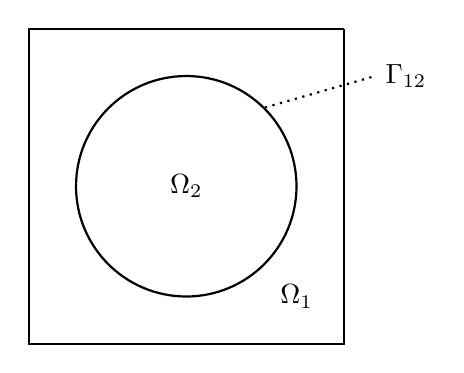
\begin{tikzpicture}[scale=2.0]
\draw[black,thick] (1,1) -- (1,-1) -- (-1,-1) -- (-1,1) -- (1,1);
\draw[black,thick] (0,0) circle (0.7);
\draw node at (0,0) {$\Omega_2$};
\draw node at (0.7,-0.7) {$\Omega_1$};
\draw[black,thick,dotted] (0.5,0.5) -- (1.2,0.7) node[anchor=west] {$\Gamma_{12}$};
\end{tikzpicture}
    \caption{the caption}
\end{figure}


Electrons in the solid phase (current collector and skeletal portion of the
porous electrode) move in response to the electric field $-\nabla \Phi_1$.

Ohm's law for the solid phase reads
\begin{equation}
    i_1 = -\sigma \nabla \Phi_1 .
    \label{eq:ohms_law_solid_phase}
\end{equation}
$\sigma$ denotes the solid phase electronic conductivity (equal to the
inverse of the resistivity), $\Phi_1$ respresents the electric potential in
the solid phase.  The subscript $1$ indicates solid.

current in the electrolyte solution filling the pores is defined as the net flux of
charged species
\begin{equation}
    i_2 = F \sum_j \zeta_j N_j
\end{equation}
$F$ is the Faraday constant (amount of electric charge in a mole of electrons,
$F=e N_A$).  $\zeta_j$ is the charge number of species $j$

Conservation of mass to describe the motion of ionic species $j$ in the
solution filling the pores of the electrode/separator.
\begin{equation}
    \frac{\partial c_j}{\partial t} =
        -\nabla N_j + R_j
    \label{eq:nernst_planck}
\end{equation}
$R_j$ is the source term 
ions transport by migration and diffusion
Nernst-Planck relation
$N_j$ describes the flux of ions under the influence of both an ionic
concentration gradient $\nabla c_j$ and an electric field $-\nabla \Phi_2$.
\begin{equation}
N_j = -D_j (\nabla c_j - \zeta_j \frac{F}{R\Theta} c_j \nabla \Phi_2)
\end{equation}
$\frac{\zeta_j F c_j}{R \Theta}$ represents the mobility of the ions, i.e.
their ability to move in the solution in response to the electric field
$-\Phi_2$.  $R$ is universal gas constant.
$\Theta$ is the absolute temperature in K.


the movement of charged species in the solution
$\kappa$ is used here rather than $\sigma$ to indicate that the mobile charge
carriers in the electrolyte are ions as opposed to electrons in the metal
portion.

In many supercapacitor and battery systems, the electrolyte can be considered
to be a binary mixture \cite{Newman2004}.  Following \cite{Verbrugge2005}, we
assume a binary 1:1 electrolyte, i.e. $j=+,-$ and $\zeta_+=-\zeta_-=1$.
(\cite{Verbrugge2005} says it is consistent with electrolytes employed in
supercapacitor systems)
$\frac{d q_+}{d q}=\frac{d q_-}{d q}=-\frac{1}{2}$

electroneutrality dictates that $\sum_j \zeta_j c_j = 0$ in the electrolyte.
$c_+=c_-=c$

Current is associated with the flux of ions $i_2 = F(N_+ - N_-)$

\begin{equation}
    \kappa = \frac{F^2}{RT} \frac{1}{2} D \left(
        \frac{1}{t_-} + \frac{1}{t_+}
        \right) c
\end{equation}

the binary diffusion coefficient $D$ is an average of the individual ionic
diffusivities 
\begin{equation}
    D = \frac{2 D_+ D_-}{D_+ + D_-} ,
\end{equation}
and the transference number is defined as
\begin{equation}
    t_+ = \frac{D_+}{D_+ + D_-}
    , \quad
    t_- = \frac{D_-}{D_+ + D_-}
    , \quad \text{and }
    t_+ + t_- = 1 .
\end{equation}


No accumulation of charges in the solution phase
\begin{equation}
    \nabla \cdot i_2 = 0 \text{ on } \Omega_2
\end{equation}

Interface $\Gamma_{12}$
\begin{equation}
    \frac{\partial i_1}{\partial n} = 
    -\frac{\partial i_2}{\partial n} = 
        C \left( \dot{\Phi}_1 - \dot{\Phi}_2 \right)
\end{equation}
\begin{equation}
    \frac{\partial c_j}{\partial n} = 
        C \frac{d q_j}{d q} \left( \dot{\Phi}_1 - \dot{\Phi}_2 \right)
\end{equation}
$n$ is the normal vector at the solid-liquid interface pointing from 1 to 2.
[I might have messed up the signs here :D]
$\frac{d q_j}{d q}$ represents the change in surface concentration of species
$j$ assiociated with a change in the surface charge on the electrode.
$C$ is the double-layer capacity

relation between the current density and the surface overpotential
$\Phi_1-\Phi_2$ and the composition $c_j$ adjacent to the interface
$i_n = f(\Phi_1-\Phi_2,c_j) + C \left( \dot{\Phi}_1 - \dot{\Phi}_2 \right)$

first term given by Butler-Volmer equation, describes the kinetics of the
electrode reaction.  Typically we ignore it for supercapacitor modeling.

%-----------------------------------------------------------------------------
\subsection{after homogenization}
assume homogenization has somehow happened at this stage.
transport properties have been modified to take in to account porosity and
tortuosity.

\begin{equation}
    \epsilon \frac{\partial c}{\partial t} =
        \nabla \cdot \left( D \nabla c \right)
        - \frac{aC}{F} \left( 
            t_- \frac{d q_+}{d q}
            +
            t_+ \frac{d q_-}{d q}
            \right)
            \frac{\partial \left( \Phi_1 - \Phi_2 \right)}{\partial t}
\end{equation}
\begin{equation}
    \nabla \cdot i_2 =
        aC \frac{\partial \left( \Phi_1 - \Phi_2 \right)}{\partial t}
\end{equation}
$a$ is the interfacial area per unit volume.

\begin{equation}
    \rho C_p \frac{\partial \Theta}{\partial t} =
         \nabla \cdot \left( \lambda \nabla \Theta \right)
         +
         q
\end{equation}

%-----------------------------------------------------------------------------
\subsection{fe formulation}
assume
aC constant in each material layer

concentration-dependance of $\kappa$ is neglected

\newcommand{\Maa}{\langle \varphi_{i,\Phi_1}, aC \varphi_{j,\Phi_1} \rangle}
\newcommand{\Mab}{-\langle \varphi_{i,\Phi_1}, aC \varphi_{j,\Phi_2} \rangle}
\newcommand{\Mba}{-\langle \varphi_{i,\Phi_1}, aC \varphi_{j,\Phi_2} \rangle}
\newcommand{\Mbb}{\langle \varphi_{i,\Phi_1}, aC \varphi_{j,\Phi_2} \rangle}
\newcommand{\Mca}{\langle \varphi_{i,\Phi_1}, \frac{aC}{F}(t_-\frac{d q_+}{d q} + t_+\frac{d q_-}{d q}) \varphi_{j,c} \rangle}
\newcommand{\Mcb}{-\langle \varphi_{i,\Phi_1}, \frac{aC}{F}(t_-\frac{d q_+}{d q} + t_+\frac{d q_-}{d q}) \varphi_{j,c} \rangle}
\newcommand{\Mcc}{\langle \varphi_{i,c}, \epsilon \varphi_{j,c} \rangle}
\newcommand{\Mdd}{\langle \varphi_{i,\Theta}, \rho C_p \varphi_{j,\Theta} \rangle}

\begin{equation}
    M =
    \begin{pmatrix}
        \Maa & \Mab & 0    & 0    \\
        \Mba & \Mbb & 0    & 0    \\
        \Mca & \Mcb & \Mcc & 0    \\
        0    & 0    & 0    & \Mdd \\
    \end{pmatrix}
\end{equation}


\newcommand{\Kaa}{\langle \nabla\varphi_{i,\Phi_1}, \sigma \nabla\varphi_{j,\Phi_1} \rangle}
\newcommand{\Kbb}{\langle \nabla\varphi_{i,\Phi_2}, \kappa \nabla\varphi_{j,\Phi_2} \rangle}
\newcommand{\Kbc}{\langle \nabla\varphi_{i,\Phi_2}, \frac{F^2}{RT}\frac12D\left(\frac{1}{t_+}+\frac{1}{t_-}\right) \nabla\varphi_{j,\Phi_2} \rangle}
\newcommand{\Kcc}{\langle \nabla\varphi_{i,c}, D \nabla\varphi_{j,c} \rangle}
\newcommand{\Kdd}{\langle \nabla\varphi_{i,\Theta}, \lambda \nabla\varphi_{j,\Theta} \rangle}
\begin{equation}
    K =
    \begin{pmatrix}
        \Kaa  & 0    & 0    & 0 \\
        0     & \Kbb & \Kbc & 0 \\
        0     & 0    & \Kcc & 0 \\
        0     & 0    & 0    & \Kdd
    \end{pmatrix}
\end{equation}

\newpage
%-----------------------------------------------------------------------------
\section{Test case 1: constant current charge constant voltage discharge}
This is inspired by an experiment by Verbrugge et al. \cite{Verbrugge2005}.

The supercapacitor is initially fully discharged at 0 V.  Then it is charged
to 1.7 V at a constant current of 100 A.  Subsequently, a constant 1.4 V is
applied for 5 s and the supercapacitor is allowed to rest at open circuit for
3 min.  The sequence is repeated for a series of potentials from 1.8 to 2.4 V
with increments of 0.1 V.

Fig.~\ref{fig:series_of_constant_current_charge_and_constant_voltage_discharge}
illustrates that.


\begin{figure}[h!]
    \centering
    \includegraphics[width=\textwidth]{figures/series_of_constant_current_charge_and_constant_voltage_discharge}
    \caption{
Constant current charge (100 A) followed by constant voltage (1.4 V)
discharge.  The maximum voltages at the end of each charge range from 1.8 V to
2.4 V by increments of 0.1 V.  (This figure is taken from \cite{Verbrugge2005}.)
    }
    \label{fig:series_of_constant_current_charge_and_constant_voltage_discharge}
\end{figure}

\begin{figure}[h!]
    \centering
    \includegraphics[width=\textwidth]{figures/constant_current_charge_constant_voltage_discharge_current_and_voltage}
    \caption{mine}
    \label{fig:constant_current_charge_constant_voltage_discharge_current_and_voltage}
\end{figure}

\begin{figure}[h!]
    \centering
    \includegraphics[width=\textwidth]{figures/constant_current_charge_constant_voltage_discharge_power_density}
    \caption{mine}
    \label{fig:constant_current_charge_constant_voltage_discharge_current_and_voltage}
\end{figure}

\begin{figure}[h!]
    \centering
    \includegraphics[width=\textwidth]{figures/constant_current_charge_constant_voltage_discharge_temperature}
    \caption{mine}
    \label{fig:constant_current_charge_constant_voltage_discharge_temperature}
\end{figure}



%-----------------------------------------------------------------------------
\section{Test case 2: constant current cycling}
The supercapacitor undergoes a series of galvanostatic charge and discharge at
constant current 100 A over the range 1.1--2.2 V.
The experiment starts at 1.4 V with a charge.  The initial condition is
imposed by applying a potentiostatic charge from 0 V until near-equilibrium
is reached.

Fig~\ref{fig:constant_current_cycling_current_and_voltage} shows

\begin{figure}[h!]
    \centering
    \includegraphics[width=\textwidth]{figures/constant_current_cycling_current_and_voltage}
    \caption{Evolution of the potential difference between the two terminals
of the supercapacitor during the first 3 min when cycling with constant
current at 100 A between 1.1 and 2.2 V.
    }
    \label{fig:constant_current_cycling_current_and_voltage}
\end{figure}

\begin{figure}[h!]
    \centering
    \includegraphics[width=\textwidth]{figures/constant_current_cycling_power_density}
    \caption{Supercapacitor power density during constant current cycling.
Red color denotes the energy fed into the device during the charge and the
green area represents the actual energy recovered at discharge.
    }
    \label{fig:constant_current_cycling_power_density}
\end{figure}
When looking carefully at
Fig.~\ref{fig:constant_current_cycling_power_density}, one may notice that
the red and the green surface area are slightly out of balance which reflects
the dissipative energy losses in the supercapacitor due to Joule heating.
The ratio between green to red surface area over one charge/discharge cycle
gives the efficiency $\eta = 85.8\%$.  The heat produced makes the temperature
field in the supercapacitor rise.  Its maximum value is plotted in
Fig.~\ref{fig:constant_current_cycling_temperature} as a function of time.


\begin{figure}[h!]
    \centering
    \includegraphics[width=\textwidth]{figures/constant_current_cycling_temperature}
    \caption{Evolution of the maximum temperature in the supercapacitor over
1 hour of cycles charge/discharge at 100 A.  0 represents the ambient
temperature.
    }
    \label{fig:constant_current_cycling_temperature}
\end{figure}

%-----------------------------------------------------------------------------
\section{Test case 3: constant power}





\bibliographystyle{plain}
\bibliography{mybib}

\end{document}  
